\documentclass[11pt,a4paper]{article}
\usepackage[margin=19mm,top=20mm,bottom=20mm]{geometry}
\usepackage{amsmath,amssymb,graphicx,array,fancyhdr,lastpage,textcomp,fancyvrb}
\usepackage{fontspec}
\usepackage[hidelinks]{hyperref}
\setmainfont{texgyreheros-regular.otf}[BoldFont=texgyreheros-bold.otf,ItalicFont=texgyreheros-italic.otf,BoldItalicFont=texgyreheros-bolditalic.otf]
\setmonofont{lmmono10-regular.otf}
\setlength{\parindent}{0pt}\setlength{\parskip}{5pt}
\setlength{\headheight}{14pt}
\pagestyle{fancy}\fancyhf{}
\renewcommand{\headrulewidth}{0.3pt}\renewcommand{\footrulewidth}{0.3pt}
\fancyfoot[L]{\footnotesize by paper.shrit.in\quad |\quad normal}
\fancyfoot[R]{\footnotesize Page \thepage\ of \pageref{LastPage}}
\begin{document}
\fancyhead[L]{\small Discrete Mathematical Structures}\fancyhead[R]{\small Set A: Ensemble}
{\LARGE\bfseries Worked Solutions}\par{\large Discrete Mathematical Structures}\par\textbf{Set A: Ensemble | CSE Semester 3}\par
Companion to \texttt{dms-ensemble.pdf}. Question numbers match that paper. Equivalent correct methods are acceptable. These are independent worked solutions, not an official university marking scheme.\par\medskip\hrule\medskip
Questions 1--5: MCQ answer key, 1 mark each (5 marks total). Questions 6 onward: theory solutions (25 marks total).\par
\noindent\begin{minipage}{\linewidth}\subsection*{1. Complement conditions}
\textbf{Correct option: (B).} A complement joins with the element to give 1 and meets with it to give 0.
\end{minipage}\par\medskip
\noindent\begin{minipage}{\linewidth}\subsection*{2. Complement uniqueness}
\textbf{Correct option: (D).} Complement existence is a Boolean-algebra property, and distributivity gives uniqueness.
\end{minipage}\par\medskip
\noindent\begin{minipage}{\linewidth}\subsection*{3. Boolean simplification}
\textbf{Correct option: (A).} Distribution gives $(a\lor\neg a)\land(a\lor b)=1\land(a\lor b)=a\lor b$.
\end{minipage}\par\medskip
\noindent\begin{minipage}{\linewidth}\subsection*{4. Disjunctive normal form}
\textbf{Correct option: (C).} $(x\land y)\lor(\neg x\land z)$ is an OR of two AND terms of literals.
\end{minipage}\par\medskip
\noindent\begin{minipage}{\linewidth}\subsection*{5. Conjunctive normal form}
\textbf{Correct option: (B).} $(x\lor y)\land(\neg x\lor z)$ is an AND of two OR clauses of literals.
\end{minipage}\par\medskip
\noindent\begin{minipage}{\linewidth}\subsection*{6. Divisibility poset and antichains}

The cover relations are $(1,2),(1,3),(2,12),(2,18),(3,12),(3,18),(12,36),(18,36)$. They determine the Hasse diagram below; line crossings without a labelled vertex are not additional elements.
\begin{center}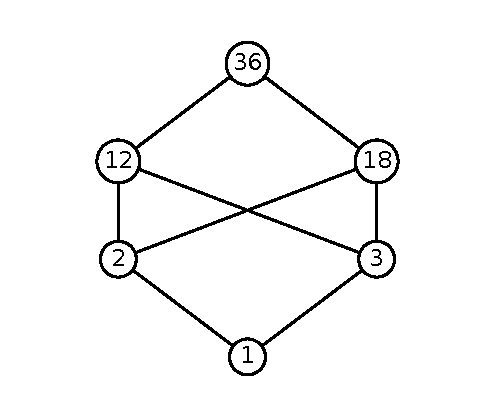
\includegraphics[width=.48\linewidth]{figures/hasse-ensemble.pdf}\end{center}
This poset is \textbf{not a lattice}. The common upper bounds of 2 and 3 are 12, 18 and 36. The two minimal common upper bounds 12 and 18 are incomparable, so there is no least upper bound. Equivalently, 12 and 18 have no greatest lower bound in the set: 2 and 3 are incomparable maximal common lower bounds. It is not valid to import gcd 6 into the set, since 6 is absent.

The complete list of antichains with more than one element is $\boxed{\{2,3\},\ \{12,18\}}$. Every other distinct pair is comparable, so there are no larger antichains.
\end{minipage}\par\medskip
\noindent\begin{minipage}{\linewidth}\subsection*{7. Bounded item selection}

Let $u=A-1$, $v=B-3$, $w=C-5$. Then $u+v+w=6$, with $0\le u\le3$, $0\le v\le4$, $0\le w\le5$. The unrestricted nonnegative count is $\binom82=28$.

Subtract violations: $u\ge4$ contributes $\binom42=6$, $v\ge5$ contributes $\binom32=3$, and $w\ge6$ contributes $\binom22=1$. Intersections are impossible because their minimum sums exceed 6. Thus
\[\boxed{28-6-3-1=18}.\]
Items of the same type are indistinguishable, so this counts feasible triples of quantities, not arrangements.
\end{minipage}\par\medskip
\noindent\begin{minipage}{\linewidth}\subsection*{8. Partition bijection}

For positive n, let $\lambda$ be a partition of n with every part at least 3. In its Ferrers diagram, the first three columns have the same height k. Its conjugate partition $\mu=\lambda'$ therefore satisfies $\mu_1=\mu_2=\mu_3=k$.

Define a new partition
\[\nu=(\mu_1+2,\mu_2+1,\mu_3,\mu_4,\ldots).
\]
Its total is $n+3$, and its three largest parts are $k+2,k+1,k$, which are consecutive.

Conversely, if a partition of $n+3$ has largest parts $k+2,k+1,k$, subtract 2 from the first part and 1 from the second. The resulting partition has three equal largest parts k and total n. Conjugating it gives a partition of n in which every row has at least three cells, hence every part is at least 3. These constructions undo each other, proving the claimed equality. For n=1 or 2, both sets are empty.
\end{minipage}\par\medskip
\noindent\begin{minipage}{\linewidth}\subsection*{9. The 75th Fike permutation}

Use the original descending-exchange Fike convention, with the original arrangement 01234 counted as permutation 1. Enumerate $(d_2,d_3,d_4,d_5)$ with $d_k=k,k-1,\ldots,1$, and $d_5$ varying fastest. For each tuple, start from 01234 and exchange positions k and $d_k$ in increasing k order, using one-based positions.

The zero-based index is $75-1=74$. The block weights for these four choices are 60, 20, 5 and 1:
\[74=1(60)+0(20)+2(5)+4(1).
\]
Thus $(d_2,d_3,d_4,d_5)=(2-1,3-0,4-2,5-4)=\boxed{(1,3,2,1)}$.
\begin{center}\renewcommand{\arraystretch}{1.2}\begin{tabular}{ll}\hline Exchange & Arrangement\\\hline
Start & 01234\\
Positions 2 and 1 & 10234\\
Positions 3 and 3 & 10234\\
Positions 4 and 2 & 13204\\
Positions 5 and 1 & 43201\\\hline\end{tabular}\end{center}
Hence the answer under this convention is $\boxed{43201}$.

{\small Convention reference: J. S. Rohl, ``Programming Improvements to Fike's Algorithm for Generating Permutations,'' The Computer Journal 19(2), 156--159 (1976), Figure 1 and recursive procedure. \url{https://doi.org/10.1093/comjnl/19.2.156}. The convention is stated explicitly because Fike order is not lexicographic order.}
\end{minipage}\par\medskip
\noindent\begin{minipage}{\linewidth}\subsection*{10. Regular self-complementary graph}

Assume a nonempty simple graph. If G is r-regular on n vertices, its complement is $(n-1-r)$-regular. Isomorphism to its complement implies
\[r=n-1-r,\qquad r=(n-1)/2.
\]
Therefore n is odd. The handshake lemma says $nr=2|E|$ is even. Since n is odd, r must be even; write $r=2t$. Substitution gives $n=2r+1=\boxed{4t+1}$, with $t\ge0$.
\end{minipage}\par\medskip
\noindent\begin{minipage}{\linewidth}\subsection*{11. Minimum degree forces connectivity}

Suppose G is disconnected, and a component has s vertices. A vertex in that component has degree at most $s-1$, so
\[s-1\ge\delta(G)\ge(p-1)/2,\quad s\ge(p+1)/2.
\]
Every component must satisfy this bound. Two components would already contain at least $p+1$ vertices, contradicting the total p. Hence G is connected. This argument assumes the usual simple-graph setting; a one-vertex graph is connected directly.
\end{minipage}\par\medskip
\noindent\begin{minipage}{\linewidth}\subsection*{12. Dijkstra on the directed source network}

Respect arrow direction. The outgoing edges are:
$v_1\to v_2:4$, $v_1\to v_3:5$;
$v_2\to v_1:6$, $v_2\to v_3:4$, $v_2\to v_5:8$;
$v_3\to v_2:6$, $v_3\to v_4:2$, $v_3\to v_6:3$;
$v_4\to v_5:7$;
$v_5\to v_1:3$, $v_5\to v_4:2$;
$v_6\to v_3:5$, $v_6\to v_4:4$.
The table records tentative distances after relaxing outgoing edges of each settled vertex.
\begin{center}\renewcommand{\arraystretch}{1.2}\begin{tabular}{lllllll}\hline Settled & $d_1$ & $d_2$ & $d_3$ & $d_4$ & $d_5$ & $d_6$\\\hline
Initial & 0 & $\infty$ & $\infty$ & $\infty$ & $\infty$ & $\infty$\\
$v_1$ & 0 & 4 & 5 & $\infty$ & $\infty$ & $\infty$\\
$v_2$ & 0 & 4 & 5 & $\infty$ & 12 & $\infty$\\
$v_3$ & 0 & 4 & 5 & 7 & 12 & 8\\
$v_4$ & 0 & 4 & 5 & 7 & 12 & 8\\
$v_6$ & 0 & 4 & 5 & 7 & 12 & 8\\
$v_5$ & 0 & 4 & 5 & 7 & 12 & 8\\\hline\end{tabular}\end{center}\begin{center}\renewcommand{\arraystretch}{1.2}\begin{tabular}{lll}\hline Destination & Shortest path & Length\\\hline
$v_1$ & $v_1$ & 0\\
$v_2$ & $v_1\to v_2$ & 4\\
$v_3$ & $v_1\to v_3$ & 5\\
$v_4$ & $v_1\to v_3\to v_4$ & 7\\
$v_5$ & $v_1\to v_2\to v_5$ & 12\\
$v_6$ & $v_1\to v_3\to v_6$ & 8\\\hline\end{tabular}\end{center}
\end{minipage}\par\medskip

\end{document}
